\chapter{Softwaretechnik}

Zusammenfassung der Vorlesung "`Softwaretechnik 2"' aus dem Wintersemester 2016.\footnote{\url{https://sdqweb.ipd.kit.edu/wiki/Vorlesung_Softwaretechnik_II_WS16/17}}

\section{Einführung}

\section{Gesetzmäßigkeiten}
\begin{itemize}
	\item \textit{Brook's Law}: "`Adding manpower to a late software projcet makes it later."'
	\item \textit{Boehm's Law}: "`Errors are more frequent during requirements and design."'
	\item \textit{Dijkstra 1969}: "`Testing shows the presence, not the absende of bugs."'
	\item (One of) \textit{Lehman's Laws}: "`A system that is used will be changed."'
	\item \textit{Parnas' Law}: "`Only what is hidden can be chaned without risk"' (\(\rightarrow\) Kapselung notwendig)
\end{itemize}



\section{Software-Entwicklungsprozess}

\begin{itemize}
	\item Vorgehensmodell: Abstrakte Beschreibung eines Software-Entwicklungsprozesses. Beinhaltet Richtlinien bezüglich Aktivitäten, Rollen und Ergebnissen (Artefakte, Dokumente, etc.)
	\item "`Code and Fix"', als Vorgehensmodell unzureichend, da es zu schlecht strukturierten und dokumentierten Programmen führt
	\item \textbf{Wasserfallmodell}
	\begin{itemize}
		\item Phasen und Ergebnisse der Phasen
		\begin{enumerate}
			\item Planung: Lastenheft, Projektplan, Kalkulation
			\item Definition: Pflichtenheft, GUI-Beschreibung, eventuell Benutzerhandbuch
			\item Entwurf: Enwurfsdokumente, Modulführer
			\item Implementierung: Komponenten und Dokumentation, Testeinrichtung
			\item Testen
			\item Einsatz und Wartung: "`Fertiges"' System
		\end{enumerate}
		\item Probleme
		\begin{itemize}
			\item Große Softwareprojekte können i.d.R. nicht komplett (auf mehrere Jahre) geplant werden
			\item Abgrenzung der einzelnen Phasen in der Praxis oft unrealistisch
			\item Zu unflexibel bezüglich Änderungen oder Rückschritten
		\end{itemize}
	\end{itemize}
	\item \textbf{V-Modell} \\\\
		\begin{minipage}{\linewidth}
			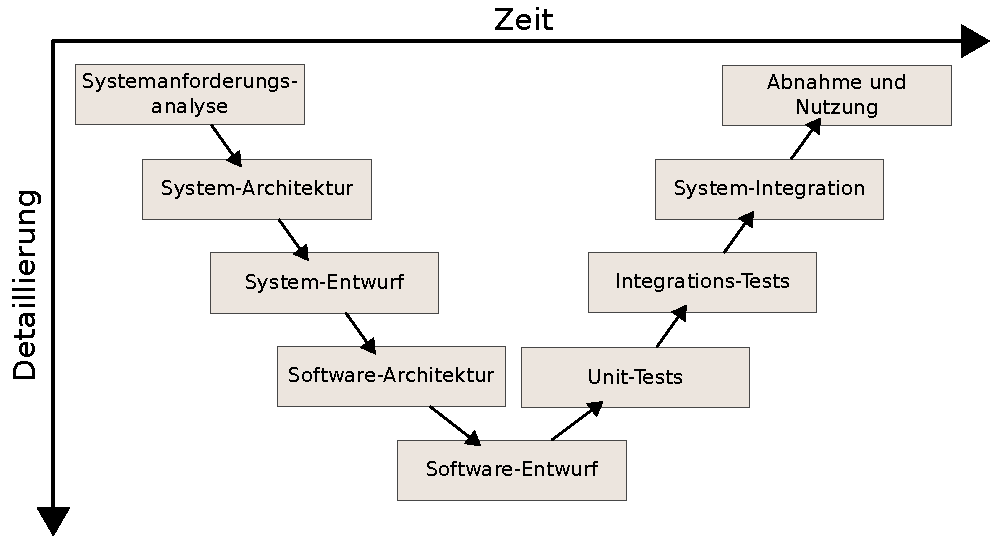
\includegraphics[scale=0.8]{swt2/V-Modell.pdf}
		\end{minipage}
\end{itemize}